\documentclass{beamer}
\usepackage{graphicx}
\usepackage{verbatim}
\usepackage{amsmath}
\usepackage{amsfonts}
\usepackage{setspace}
% \usepackage{beamerthemesplit} // Activate for custom appearance

\title{Inference in Regression Analysis}
\author{Dr. Frank Wood}

\date{}

\DeclareMathOperator*{\Ave}{\mathbb{E}}
\DeclareMathOperator*{\Var}{Var}

\begin{document}

\frame{\titlepage}



\frame[t] {
 \frametitle{Inference in the Normal Error Regression Model}
$$Y_i = \beta_0 + \beta_1 X_i + \epsilon_i$$
\begin{itemize}
\item $Y_i$ value of the response variable in the $i^{th}$ trial
\item $\beta_0$ and $\beta_1$ are parameters
\item $X_i$ is a known constant, the value of the predictor variable in the $i^{th}$ trial
\item $\epsilon_i \sim_{iid} N(0,\sigma^2)$
\item $i = 1,\ldots,n$
\end{itemize}
}

\frame[t] {
 \frametitle{Inference concerning $\beta_1$}
Tests concerning $\beta_1$ (the slope) are often of interest,
particularly
\begin{eqnarray*}
H_0 : \beta_1 &=& 0 \\
H_a: \beta 1 &\neq& 0
\end{eqnarray*}
the null hypothesis model$$Y_i = \beta_0 + (0) X_i + \epsilon_i$$
implies that there is no relationship between Y and X.\\
\bigskip

Note the means of all the $Y_i$'s are equal at all levels of $X_i$.
 }

\frame[t] {
 \frametitle{Quick Review : Hypothesis Testing}
\begin{itemize}
\item Elements of a statistical test

\begin{itemize}
\item Null hypothesis, $H_0$
\item Alternative hypothesis, $H_a$
\item Test statistic
\item Rejection region
\end{itemize}
\end{itemize}
}

\frame[t] {
 \frametitle{Quick Review : Hypothesis Testing - Errors}
\begin{itemize}
\item Errors

\begin{itemize}
\item A type I error is made if $H_0$ is rejected when $H_0$ is true.  The probability of a type I error is denoted by $\alpha$.  The value of $\alpha$ is called the level of the test.
\item A type II error is made if $H_0$ is accepted when $H_a$ is true.  The
probability of a type II error is denoted by $\beta$.
\end{itemize}
\end{itemize}
}

\frame[t] {
 \frametitle{P-value}
The p-value, or attained significance level, is the smallest level
of significance $\alpha$ for which the observed data indicate that
the null hypothesis should be rejected. }

\frame[t] {%%%change pic%%%
 \frametitle{Null Hypothesis}
If the null hypothesis is that $\beta_1 = 0$ then $b_1$ should fall in
the range around zero.  The further it is from $0$ the less likely the null hypothesis is to hold.
\begin{figure}
  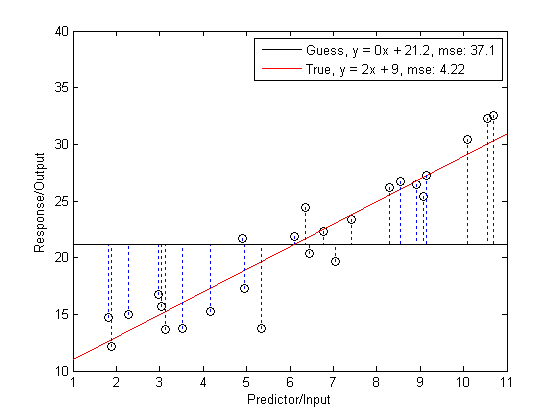
\includegraphics[height=60mm]{b1.png}
\end{figure}
}

\frame[t] {%%%change pic%%%
 \frametitle{Alternative Hypothesis : Least Squares Fit}
 If we find that our estimated value of $b_1$ deviates from $0$ then we have to determine whether or not that deviation would be surprising given the model and the sampling distribution of the estimator.  If it is sufficiently (where we define what sufficient is by a confidence level) different then we reject the null hypothesis.
\begin{figure}
  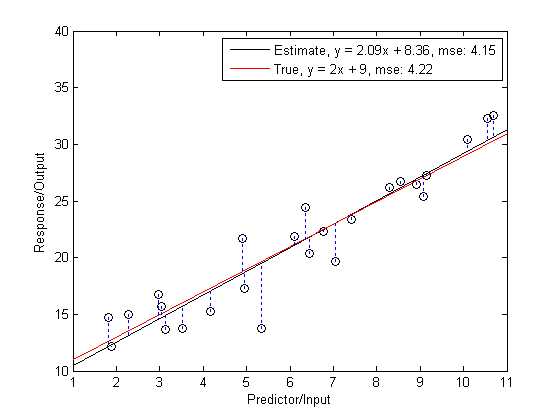
\includegraphics[height=50mm]{alternative.png}
\end{figure}
}

\frame[t] {
 \frametitle{Testing This Hypothesis}
\begin{itemize}
\item Only have a finite sample
\item Different finite set of samples (from the same population / source) will (almost always) produce different point estimates of $\beta_0$ and $\beta_1$ $(b_0, b_1)$ given the same estimation procedure
\item Key point: $b_0$ and $b_1$ are random variables whose sampling distributions can be statistically characterized
\item Hypothesis tests about $\beta_0$ and $\beta_1$ can  be constructed using these distributions.
\item The same techniques for deriving the sampling distribution of ${\bf b} = [b_0, b_1]$ are used in multiple regression.
\end{itemize}
}

\frame[t] {
 \frametitle{Sampling Dist. Of $b_1$}
\begin{itemize}
\item The point estimator for $b_1$ is
\begin{eqnarray*}
b_1 &=& \frac{\sum(X_i - \bar X)(Y_i - \bar Y)}{\sum(X_i-\bar X)^2} \\
%b_0 &=& \bar Y - b_1 \bar X\\
%\bar X &=& \frac{\sum X_i}{n} \\
%\bar Y&=&\frac{\sum Y_i}{n}
\end{eqnarray*}
\item The sampling distribution for $b_1$ is the distribution of $b_1$ that arises from the variability of $b_1$ when the predictor variables $X_i$ are held fixed and the observed outputs are repeatedly sampled
\item Note that the sampling distribution we derive for $b_1$ will be highly dependent on our modeling assumptions.
\end{itemize}
}

\frame[t] {
 \frametitle{Sampling Dist. Of $b_1$ In Normal Regr. Model }
\begin{itemize}
\item For a normal error regression model the sampling distribution of $b_1$ is normal, with mean and variance given by
\begin{eqnarray*}
\Ave(b_1) &=& \beta_1\\
\Var(b_1) &=& \frac{\sigma^2}{\sum(X_i-\bar X)^2}
\end{eqnarray*}

\item To show this we need to go through a number of algebraic steps.

\end{itemize}
}

\frame[t] {
 \frametitle{First step}
To show
$$\sum(X_i - \bar X)(Y_i - \bar Y) = \sum(X_i - \bar X)Y_i$$
we observe
\begin{eqnarray*}
\sum(X_i - \bar X)(Y_i - \bar Y) &=& \sum(X_i - \bar X)Y_i - \sum(X_i - \bar X)\bar Y \\
&=& \sum(X_i - \bar X)Y_i - \bar Y \sum(X_i - \bar X) \\
&=& \sum(X_i - \bar X)Y_i - \bar Y \sum(X_i) + \bar Y n \frac{\sum X_i}{n} \\
&=& \sum(X_i - \bar X)Y_i
\end{eqnarray*}
}

\frame[t] {
 \frametitle{$b_1$ as convex combination of $Y_i$'s}
$b_1$ can be expressed as a linear combination of the $Y_i's$
\begin{eqnarray*}
b_1 &=& \frac{\sum(X_i - \bar X)(Y_i - \bar Y)}{\sum(X_i-\bar X)^2} \\
&=& \frac{\sum(X_i - \bar X)Y_i}{\sum(X_i-\bar X)^2}  \;\;\;\;\; \mbox{from previous slide} \\
&=& \sum k_i Y_i
\end{eqnarray*}
where $$k_i = \frac{(X_i - \bar X)}{\sum(X_i-\bar X)^2}$$ }

\frame[t] {
 \frametitle{Properties of the $k_i's$}
It can be shown that
\begin{eqnarray*}
\sum k_i &=& 0 \\
\sum k_i X_i &=& 1 \\
\sum k_i^2 &=& \frac{1}{\sum(X_i - \bar X)^2}
\end{eqnarray*}
(possible homework).  We will use these properties to prove various
properties of the sampling distributions of $b_1$ and $b_0$.

}

\frame[t] {
 \frametitle{Normality of $b_1's$ Sampling Distribution}
\begin{itemize}
\item Useful fact:
\begin{itemize}
\item A linear combination of independent normal random variables is normally distributed
\item More formally: when $Y_1,\ldots,Y_n$ are independent normal random variables, the linear combination
$a_1Y_1 + a_2Y_2 + \ldots + a_nY_n$ is normally distributed, with
mean $\sum a_i\Ave(Y_i)$ and variance $\sum a_i^2\Var(Y_i)$
\end{itemize}
\end{itemize}
}

\frame[t] {
 \frametitle{Normality of $b_1's$ Sampling Distribution}
Since $b_1$ is a linear combination of the $Y_i's$ and each $Y_i$ is
an independent normal random variable, then $b_1$ is distributed
normally as well
\begin{eqnarray*}
b_1 &=& \sum k_i Y_i, \, k_i = \frac{(X_i - \bar X)}{\sum(X_i-\bar
X)^2}
\end{eqnarray*}
From previous slide
\[\Ave(b_1) = \sum k_i \Ave(Y_i), \; \; \Var(b_1) = \sum k_i^2 \Var(Y_i)\]
}

\frame[t] {
 \frametitle{$b_1$ is an unbiased estimator}
This can be seen using two of the properties
\begin{eqnarray*}
\Ave(b_1) &=& \Ave(\sum k_i Y_i) \\
&=& \sum k_i \Ave(Y_i) \\
&=& \sum k_i (\beta_0+\beta_1 X_i) \\
&=& \beta_0 \sum k_i + \beta_1 \sum k_i X_i \\
&=& \beta_0 (0) +  \beta_1  (1) \\
&=& \beta_1
\end{eqnarray*}
 }

\frame[t] {
 \frametitle{Variance of $b_1$}
Since the $Y_i$ are independent random variables with variance
$\sigma^2$ and the $k_i's$ are constants we get
\begin{eqnarray*}
\Var(b_1) &=& \Var(\sum k_i Y_i) = \sum k_i^2 \Var(Y_i)  \\
&=& \sum k_i^2 \sigma^2 = \sigma^2   \sum k_i^2 \\
&=& \sigma^2  \frac{1}{\sum(X_i - \bar X)^2}
\end{eqnarray*}
note that this assumes that we know $\sigma^2$. Can we?

}

\frame[t] {
 \frametitle{Estimated variance of $b_1$}
\begin{itemize}
\item When we don't know $\sigma^2$ then we have to replace it with the MSE estimate
\item Let
$$s^2 = MSE = \frac{SSE}{n-2}$$
where
$$SSE = \sum e_i^2 $$
and
$$e_i = Y_i-\hat Y_i$$
plugging in we get
\begin{eqnarray*}
\Var(b_1) &=&  \frac{\sigma^2}{\sum(X_i - \bar X)^2} \\
\hat \Var(b_1) &=&  \frac{s^2}{\sum(X_i - \bar X)^2}
\end{eqnarray*}
\end{itemize}
}

\frame[t] {
 \frametitle{Recap}
 \begin{itemize}
\item We now have an expression for the sampling distribution of $b_1$ when $\sigma^2$ is known
\begin{equation}b_1 \sim \mathcal{N}(\beta_1,  \frac{\sigma^2}{\sum(X_i - \bar X)^2})\label{b1_dist}  \end{equation} when $\sigma^2$ is known.
\item When $\sigma^2$ is unknown we have an unbiased point estimator of $\sigma^2$ 
\[\hat \Var(b_1) =  \frac{s^2}{\sum(X_i - \bar X)^2}\]
\item As $n \rightarrow \infty$ (i.e. the number of observations grows large) $\hat \Var(b_1) \rightarrow \Var(b_1)$ and we can use Eqn.~\ref{b1_dist}.
\item Questions
\begin{itemize}
\item When is $n$ big enough?
\item What if $n$ isn't big enough?
\end{itemize}

\end{itemize}


}

\frame[t] {
 \frametitle{Digression : Gauss-Markov Theorem}
In a regression model where $\Ave(\epsilon_i) = 0$ and variance $\Var(\epsilon_i) = \sigma^2 < \infty$
and $\epsilon_i$ and $\epsilon_j$ are uncorrelated for all $i$ and $j$ the least squares
estimators $b_0$ and $b_1$ are unbiased and have minimum variance among
all unbiased linear estimators.\\ Remember
\begin{eqnarray*}
b_1 &=& \frac{\sum(X_i - \bar X)(Y_i - \bar Y)}{\sum(X_i-\bar X)^2} \\
b_0 &=& \bar Y - b_1 \bar X
%\bar X &=& \frac{\sum X_i}{n} \\
%\bar Y&=&\frac{\sum Y_i}{n}
\end{eqnarray*}

}


\frame[t] {
 \frametitle{Proof}
\begin{itemize}
\item The theorem states that $b_1$ as minimum variance among all unbiased linear estimators of the form
$$\hat \beta_1 = \sum c_i Y_i$$
\item As this estimator must be unbiased we have
\begin{eqnarray*}
\Ave(\hat \beta_1) &=& \sum c_i \Ave(Y_i) = \beta_1 \\
 &=& \sum c_i  (\beta_0 + \beta_1 X_i) = \beta_0 \sum c_i  + \beta_1 \sum c_i X_i  = \beta_1
\end{eqnarray*}
\end{itemize}
}

\frame[t] {
 \frametitle{Proof cont.}
\begin{itemize}
\item Given these constraints
\begin{eqnarray*}
\beta_0 \sum c_i  + \beta_1 \sum c_i X_i  = \beta_1
\end{eqnarray*}
clearly it must be the case that $\sum c_i =0$ and $\sum c_iX_i = 1$

\item The variance of this estimator is
\begin{eqnarray*}
\Var(\hat \beta_1) &=& \sum c_i^2 \Var(Y_i) = \sigma^2 \sum c_i^2
\end{eqnarray*}

\end{itemize}
}

\frame[t] {
 \frametitle{Proof cont.}
Now define $c_i = k_i + d_i$ where the $k_i$ are the constants we
already defined and the $d_i$ are arbitrary constants.  Let's look
at the variance of the estimator
\begin{eqnarray*}
\Var(\hat \beta_1) &=& \sum c_i^2 \Var(Y_i) = \sigma^2 \sum (k_i+d_i)^2 \\
&=& \sigma^2(\sum k_i^2 + \sum d_i^2 + 2 \sum k_i d_i)
\end{eqnarray*}
Note we just demonstrated that $$\sigma^2 \sum k_i^2 = \Var(b_1)$$}

\frame[t] {
 \frametitle{Proof cont.}
Now by showing that $\sum k_id_i = 0$ we're almost done
\begin{eqnarray*}
 \sum k_i d_i &=& \sum k_i (c_i - k_i) \\
&=& \sum k_i (c_i - k_i) \\
&=& \sum k_i c_i - \sum k_i^2 \\
&=& \sum c_i \left(\frac{X_i - \bar X}{\sum(X_i - \bar X)^2}\right) - \frac{1}{\sum(X_i - \bar X)^2} \\
&=&  \frac{\sum c_i X_i - \bar X\sum c_i}{\sum(X_i - \bar X)^2} -
\frac{1}{\sum(X_i - \bar X)^2} = 0
\end{eqnarray*}
}

\frame[t] {
 \frametitle{Proof end}
So we are left with \begin{eqnarray*}
\Var(\hat \beta_1) &=& \sigma^2(\sum k_i^2 + \sum d_i^2 ) \\
&=& \Var(b_1) + \sigma^2(\sum d_i^2 )
\end{eqnarray*}
which is minimized when the $d_i's = 0$. This means that the least
squares estimator $b_1$ has minimum variance among all unbiased linear
estimators.
 }

\frame[t] {
 \frametitle{Sampling Distribution of $(b_1 - \beta_1)/S(b_1)$}
\begin{itemize}
\item $b_1$ is normally distributed so $(b_1-\beta_1)/(\sqrt{\Var(b_1)})$ is a standard normal variable
\item We don't know $\Var(b_1)$ so it must be estimated from data.  We have already denoted it's estimate
\item If using the estimate $\hat V(b_1)$ it can be shown that
$$\frac{b_1-\beta_1}{\hat{S}(b_1)} \sim t(n-2)$$
$$\hat S(b_1) = \sqrt{ \hat V(b_1)}$$
\end{itemize}
}

\frame[t] {
 \frametitle{Where does this come from?}
\begin{itemize}
\item For now we need to rely upon the following theorem\\
\bigskip
For the normal error regression model
$$\frac{SSE}{\sigma^2} = \frac{\sum (Y_i - \hat Y_i)^2}{\sigma^2} \sim \chi^2(n-2)$$
and is independent of $b_0$ and $b_1$\\
\bigskip
\item Intuitively this follows the standard result for the sum of squared normal random
variables
\item Here there are two linear constraints imposed by the regression
parameter estimation that each reduce the number of degrees of
freedom by one.
\item We will revisit this subject soon.


\end{itemize}
}

\frame[t] {
 \frametitle{Another useful fact : t distributed random variables}
Let z and $\chi^2(\nu)$ be independent random variables (standard
normal and $\chi^2$ respectively).  The following random variable is a t-dstributed random
variable:
$$t(\nu) = \frac{z}{\sqrt{\frac{\chi^2(\nu)}{\nu}}}$$
This version of the t distribution has one parameter, the degrees of
freedom $\nu$

}

\frame[t] {
 \frametitle{Distribution of the studentized statistic}
To derive the distribution of this statistic, first we do the
following rewrite
$$\frac{b_1 - \beta_1}{{\hat S(b_1)}} = \frac{\frac{b_1 - \beta_1}{{ S(b_1)}}}{\frac{\hat S(b_1)}{ S(b_1)}}$$
$$\frac{\hat S(b_1)}{ S(b_1)} = \sqrt{\frac{\hat V(b_1)}{ \Var(b_1)}}$$}

\frame[t] {
 \frametitle{Studentized statistic cont.}
And note the following
$$\frac{\hat V(b_1)}{ \Var(b_1)} = \frac{\frac{MSE}{\sum(X_i-\bar X)^2}}{\frac{\sigma^2}{\sum(X_i-\bar X)^2}} = \frac{MSE}{\sigma^2} = \frac{SSE}{\sigma^2(n-2)}$$
where we know (by the given theorem) the distribution of the last
term is $\chi^2$ and indep. of $b_1$ and $b_0$
$$\frac{SSE}{\sigma^2(n-2)} \sim \frac{\chi^2(n-2)}{n-2}$$}

\frame[t] {
 \frametitle{Studentized statistic final}
But by the given definition of the t distribution we have our result
$$\frac{b_1-\beta_1}{\hat{S}(b_1)} \sim t(n-2)$$
because putting everything together we can see that $$\frac{b_1 -
\beta_1}{\hat S(b_1)} \sim
\frac{z}{\sqrt{\frac{\chi^2(n-2)}{n-2}}}$$ }

\frame[t] {
 \frametitle{Confidence Intervals and Hypothesis Tests}
Now that we know the sampling distribution of $b_1$ (t with n-2
degrees of freedom) we can construct confidence intervals and
hypothesis tests easily 
\bigskip
Things to think about
\begin{itemize}
\item What does the t-distribution look like?
\item Why is the estimator distributed according to a t-distribution rather than a normal distribution?
\item When performing tests why does this matter?
\item When is it safe to cheat and use a normal approximation?
\end{itemize}

}


\end{document}
